%%%%%%%%%%%%%%%%%%%%%%%%%%%%%%%%%%%%%%%%%%%%%%%%%%%%%
%                                                   %
%     Penn State Colloquium Poster Template         %
%                                                   %
% Uses Penn State Colloquium class, with options:   %
%                                                   %
% Orientation:                                      %
%     portrait (default), landscape                 %
%                                                   %
% Paper size:                                       %
%     a4paper (default), a0paper, a1paper, a2paper, %
%     a3paper, a5paper, a6paper                     %
%%%%%%%%%%%%%%%%%%%%%%%%%%%%%%%%%%%%%%%%%%%%%%%%%%%%%
\documentclass{../psuposter}
\renewcommand{\templateimagepath}{../} 


%%%%%%%%%%%%%%%%%%%%%%%%%%%%%%%%%%%%%%%%%%%%%%%%%%%%%
%               Package Dependencies                %
%%%%%%%%%%%%%%%%%%%%%%%%%%%%%%%%%%%%%%%%%%%%%%%%%%%%%
\usepackage{natbib}
\usepackage{lipsum}                                % Dummy text
\usepackage[figwidth = 0.98\linewidth]{todonotes}  % Dummy image (and more!)
\usepackage[absolute, overlay]{textpos}            % Figure placement
\setlength{\TPHorizModule}{\paperwidth}
\setlength{\TPVertModule}{\paperheight}
\setcitestyle{numbers,square}


%%%%%%%%%%%%%%%%%%%%%%%%%%%%%%%%%%%%%%%%%%%%%%%%%%%%%
%                 AUTHOR AND TITLE                  %
%%%%%%%%%%%%%%%%%%%%%%%%%%%%%%%%%%%%%%%%%%%%%%%%%%%%%
\title{Quantum computation with noisy superconducting qubits}
\author{Abhinav Kandala \inst{1}}
\institute{\inst{1} IBM T.J. Watson Research Center}


%%%%%%%%%%%%%%%%%%%%%%%%%%%%%%%%%%%%%%%%%%%%%%%%%%%%%
%                  BEGIN DOCUMENT                   %
%%%%%%%%%%%%%%%%%%%%%%%%%%%%%%%%%%%%%%%%%%%%%%%%%%%%%
\begin{document}
\begin{frame}
\begin{columns}[t, totalwidth=\textwidth]
\begin{column}{0.45\textwidth - 1cm}


%%%%%%%%%%%%%%%%%%%%%%%%%%%%%%%%%%%%%%%%%%%%%%%%%%%%%
%                 BLOCK: BIOGRAPHY                  %
%%%%%%%%%%%%%%%%%%%%%%%%%%%%%%%%%%%%%%%%%%%%%%%%%%%%%
    \begin{block}{Speaker Biographic Summary}
    	\begin{center}
    		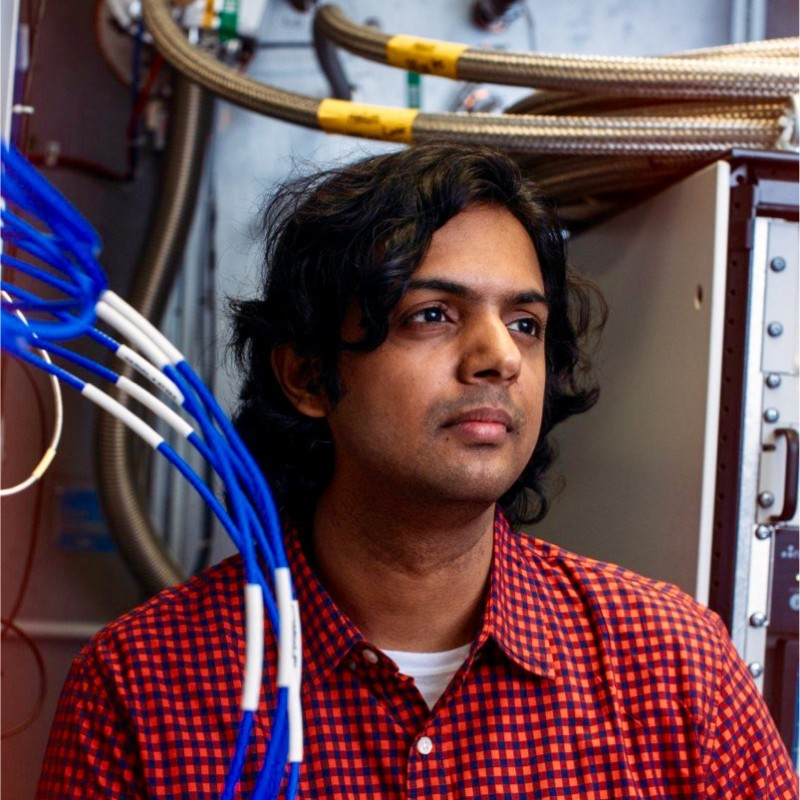
\includegraphics[width=0.6\textwidth]{images/kandala}
    	\end{center}
    	\href{}{Abhinav Kandala} is an experimental physicist in the quantum computing group at the IBM T.J. Watson Research Center. He received his Bachelors degree in Engineering Physics from the Indian institute of Technology (Bombay), and a PhD in Physics from The Pennsylvania State University, under the supervision of Prof. Nitin Samarth. Dr. Kandala went on to join the quantum computing group at IBM Research for his postdoctoral work and studied the applicability of a noisy superconducting quantum processor to simulate small molecules and quantum magnets. This work was recognized by MIT Technology Review as one of 10 Breakthrough Technologies 2018, and by C\&E News’ Research of the Year 2017. \cite{Kandala}
    \end{block}


%%%%%%%%%%%%%%%%%%%%%%%%%%%%%%%%%%%%%%%%%%%%%%%%%%%%%
%            BLOCK: RESEARCH INTERESTS              %
%%%%%%%%%%%%%%%%%%%%%%%%%%%%%%%%%%%%%%%%%%%%%%%%%%%%%
    \begin{block}{Research Interests}
        Dr. Kandala's research interests focus on the coherence and control of superconducting qubits, multi-qubit device characterization, and applications of near-term quantum computers. His prior research interests spanned exploratory semiconductors, spintronics, nano-science and solar cells, providing extensive experience with nano-fabrication, cryogenic magneto-transport, and materials characterization techniques. His most recent work has focused on error mitigation for computations performed on noisy quantum processors \cite{Kandala}
        \begin{center}
	    	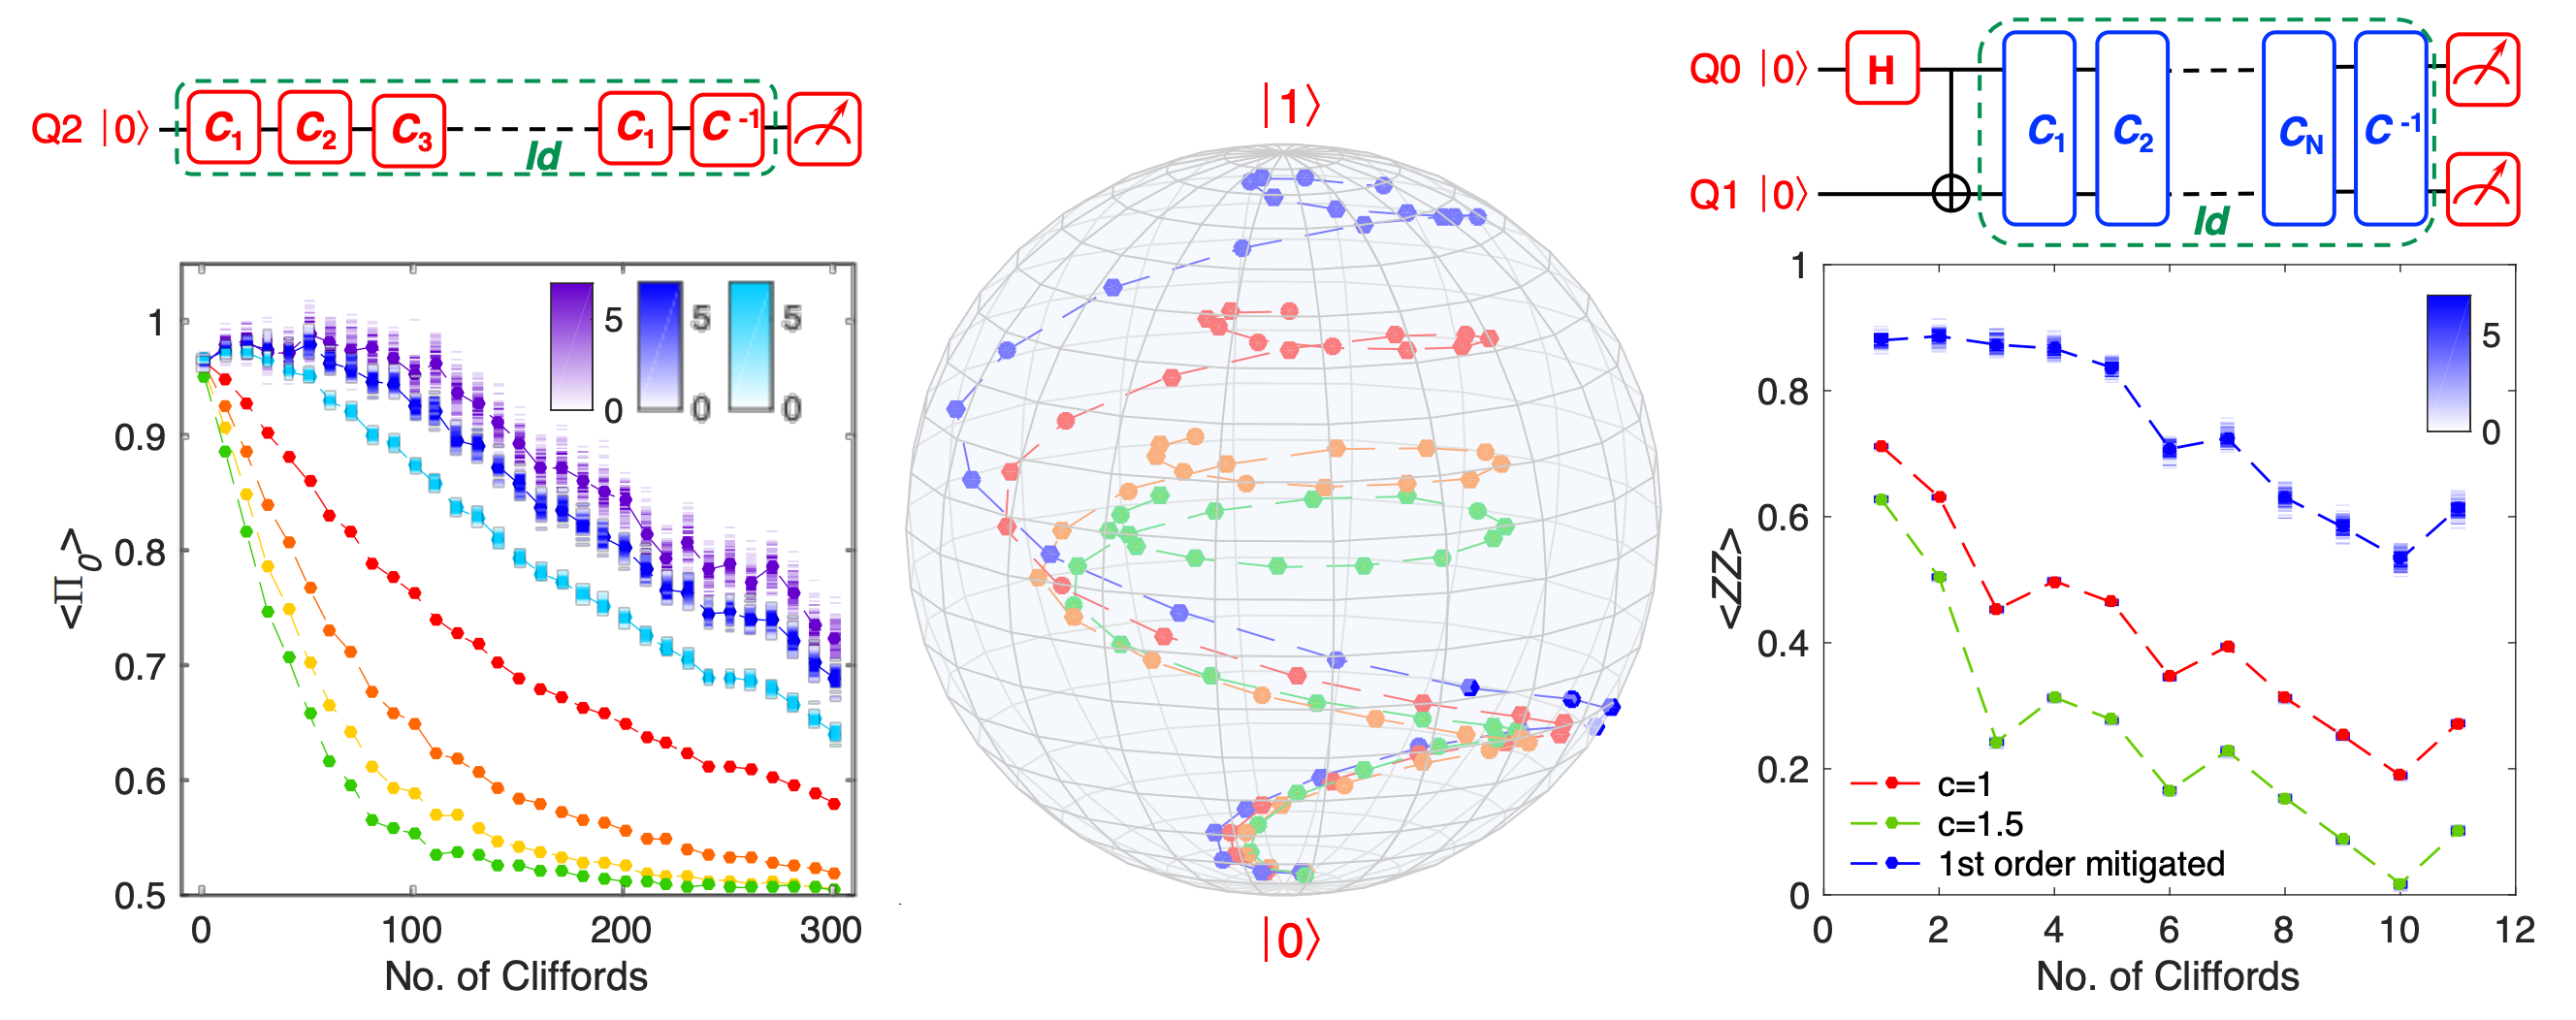
\includegraphics[width=0.98\textwidth]{images/error-mitigation}    		
    	\end{center}
    	\textit{Error mitigation of random 1-qubit and 2-qubit circuits}. \cite{kandalaExtendingComputationalReach2019}
    \end{block}
\end{column}
\begin{column}{0.55\textwidth - 1cm}


%%%%%%%%%%%%%%%%%%%%%%%%%%%%%%%%%%%%%%%%%%%%%%%%%%%%%
%                 BLOCK: ABSTRACT                   %
%%%%%%%%%%%%%%%%%%%%%%%%%%%%%%%%%%%%%%%%%%%%%%%%%%%%%
    \begin{block}{Talk Abstract}
        Improvements in the control and coherence of artificial atoms built from superconducting circuits have enabled the development of noisy processors with over 50 qubits, and the exploration of problems addressable by these devices that are intractable to classical computation. In this talk, I shall present a brief summary of superconducting qubit technology and highlight some of the dominant errors and outstanding challenges. I shall then discuss results from small-scale demonstrations of algorithms for quantum simulation. These experiments highlight the detrimental effect of decoherence and measurement errors on computations with noisy quantum processors. While this can be remedied, in theory, with quantum error correction, the resources required for its physical realization are prohibitively large for the near term. In this context, I shall introduce “error mitigation” techniques that enable access to noise-free estimates of expectation values for short depth quantum circuits, without requiring any additional hardware resources.  
    \end{block}


%%%%%%%%%%%%%%%%%%%%%%%%%%%%%%%%%%%%%%%%%%%%%%%%%%%%%
%                BLOCK: BACKGROUND                  %
%%%%%%%%%%%%%%%%%%%%%%%%%%%%%%%%%%%%%%%%%%%%%%%%%%%%%
    \begin{block}{Brief Background}
        A bit about qubits \cite{jazaeriReviewQuantumComputing2019}

        \begin{center}
		   	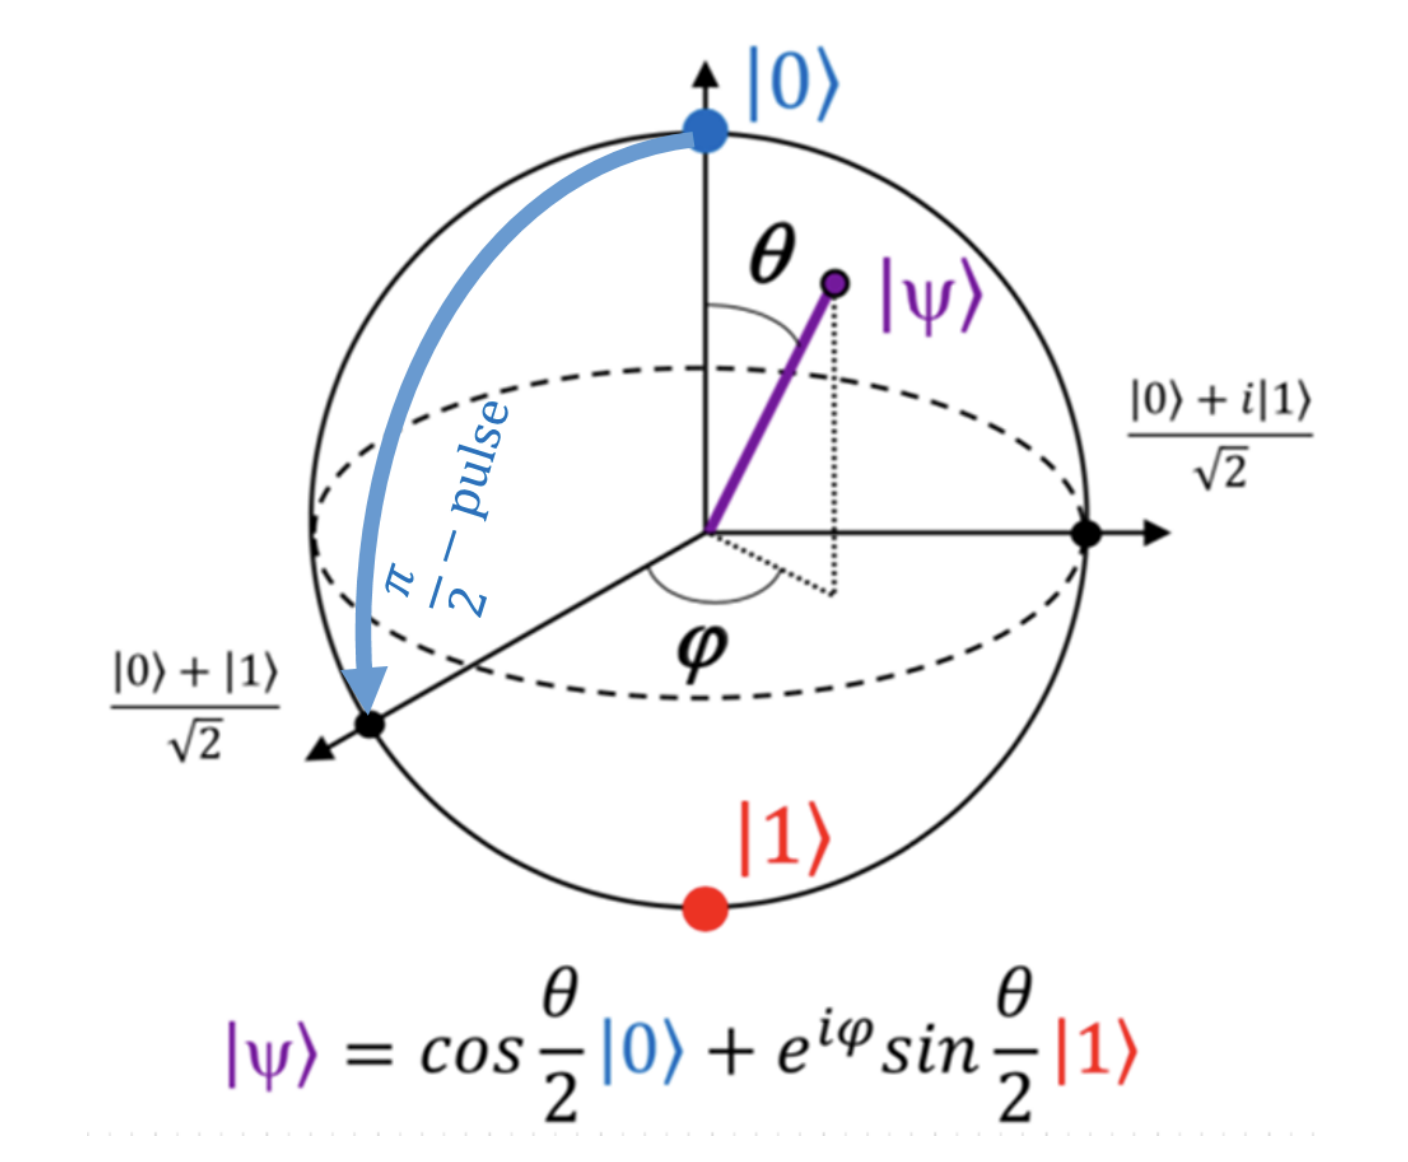
\includegraphics[width=0.55\textwidth]{images/bloch}    		
    	\end{center}
        
		Error mitigation basics \cite{kandalaExtendingComputationalReach2019}

    \end{block}


%%%%%%%%%%%%%%%%%%%%%%%%%%%%%%%%%%%%%%%%%%%%%%%%%%%%%
%                 BLOCK: REFERENCES                 %
%%%%%%%%%%%%%%%%%%%%%%%%%%%%%%%%%%%%%%%%%%%%%%%%%%%%%
    \begin{block}{References}
        \bibliographystyle{aipnum4-1}
		\bibliography{../references}
    \end{block}

\end{column}
\end{columns}


%%%%%%%%%%%%%%%%%%%%%%%%%%%%%%%%%%%%%%%%%%%%%%%%%%%%%
%                    FOOTER TEXT                    %
%%%%%%%%%%%%%%%%%%%%%%%%%%%%%%%%%%%%%%%%%%%%%%%%%%%%%
\begin{textblock}{0.5}(0.18, 0.94)
    \color{white}
    \sffamily
    \textbf{Eberly College of Science}
    \\
    Department of Physics
\end{textblock}


%%%%%%%%%%%%%%%%%%%%%%%%%%%%%%%%%%%%%%%%%%%%%%%%%%%%%
%                   END TEMPLATE                    %
%%%%%%%%%%%%%%%%%%%%%%%%%%%%%%%%%%%%%%%%%%%%%%%%%%%%%
\end{frame}
\end{document}
